\section{Интересный Haskell}
\subsection{Рекурсия}

\begin{frame}
	\tableofcontents[currentsection,currentsubsection]
\end{frame}

\begin{frame}[t,fragile]{Упражнения на рекурсию}
	% 02-01-rec.hs
	\begin{tabular}{p{0.45\linewidth}p{0.45\linewidth}}
	\centering
	Факториал:
\begin{minted}{haskell}
fac 0 = 1
fac n = n * fac (n - 1)
\end{minted}
	&
	Степень двойки: \pause
\begin{minted}{haskell}
powerOfTwo 0 = 1
powerOfTwo n = 2 *
    powerOfTwo (n - 1)
\end{minted}
	\end{tabular}
	\vspace{-10pt}

	Числа Фибоначчи: \pause
\begin{minted}{haskell}
fib n = fib' 0 1 n
fib' f1 f2 0 = a
fib' f1 f2 n = fib' f2 (f1 + f2) (n - 1)
\end{minted}
	\begin{itemize}
		\item Функции могут содержать апостроф
		\item Функции всегда должны начинаться с маленькой буквы.
		\item Мы увидели \textit{pattern matching}:
			\begin{itemize}
				\item Вместо \t{if} пишем <<шаблон>> для аргумента функции.
				\item Шаблонов может быть несколько, они проверяются сверху вниз.
				\item Приближает нас к математической нотации, избавляет от if'ов.
				\item Очень популярно в функциональных языках.
			\end{itemize}
	\end{itemize}
\end{frame}

\begin{frame}[fragile]{If не нужен}
	% 02-02-if.hs
	% 02-03-no-if.hs
\begin{minted}{haskell}
-- If
fac n = if n == 0
        then 1
        else n * fac (n - 1)
-- Pattern matching
fac 0 = 1
fac n = n * fac (n - 1)
-- If
fac_two n = if n <= 1
            then 1
            else n * fac_two (n - 2)
-- Guards
fac_two n | n <= 1    = 1
          | otherwise = n * fac (n - 2)
\end{minted}
\end{frame}

\begin{frame}[t,fragile]{Жизнь без циклов}
	Как теперь написать функцию \t{sum}? \pause
	% 02-04-sum1.hs
\begin{minted}{haskell}
sum' (x:xs) = x + sum xs
sum' _ = 0
\end{minted}
	\begin{itemize}
		\item Иногда можно делать сложный pattern matching вроде \t{x:xs} (список, первый элемент которого "--- \t{x}, а хвост "--- \t{xs}).
		\item Шаблоны всё проверяются сверху вниз, выбирается общий.
		\item Вместо имени переменной можно написать \t{\_}.
	\end{itemize}
\end{frame}

\begin{frame}[fragile]{Неявный инвариант}
	Если в императивной программе есть цикл "--- то можно вынести одну итерацию этого цикла в функцию и сделать рекурсию вместо цикла:

	\begin{tabular}{p{0.35\linewidth}p{0.55\linewidth}}
		\centering
		% 02-04-sum2.py
		% 02-04-sum2.hs
		Python & Haskell \\
\begin{minted}{python}
def sum(xs):
    a = 0
    for x in xs:
        a += x
    return a
\end{minted}
		&
\begin{minted}{haskell}
sum' xs = sum'' 0 xs
sum'' a [] = a
sum'' a (x:xs) = sum'' (a + x) xs
\end{minted}
\pause
Или так:
% 02-04-sum3.hs
\begin{minted}{haskell}
sum' xs = sum'' 0 xs
    where
        sum'' a [] = a
        sum'' a (x:xs) = ...
\end{minted}
	\end{tabular}
\end{frame}

\begin{frame}[t, fragile]{Ещё пример}
	% 02-05-uniq.py
\begin{minted}{python}
def foo(xs):
    res = []
    if not xs: return
    res.append(xs[0])
    for x in xs[1:]:
        if res[-1] != x:
            res.append(x)
    return res
\end{minted}
	Что это?
	\pause
	Удаление одинаковых значений, идущих подряд: \t{[10,~10,~20,~10]~->~[10,~20,~10]}
\end{frame}

\begin{frame}[t, fragile]{Упражнение}
	\begin{itemize}
		\item Напишите то же самое на Haskell.
		\item Возьмите код на Python в качестве основы.
		\item Преобразуйте цикл \t{for} в рекурсию. \pause
		\item Инвариант "--- последний добавленный элемент.
	\end{itemize}
	\pause
	% 02-06-uniq-imp.hs
\begin{minted}{haskell}
uniq [] = []
uniq (x:xs) = x:(uniq' x xs)
    where
        uniq' _ [] = []
        uniq' last (x:xs)
            | last == x = xs'
            | otherwise = x:xs'
            where xs' = uniq' x xs
\end{minted}
	Как-то красоты не прибавилось.
\end{frame}

\begin{frame}{И где золотые горы?}
	\begin{center}
		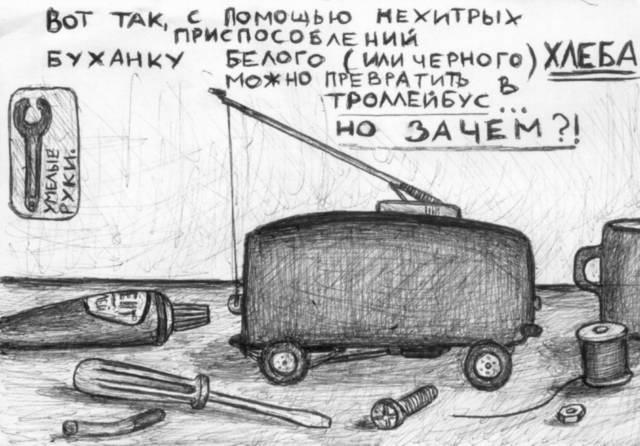
\includegraphics[scale=0.35]{bread-why.jpg}
	\end{center}
	Мы пока написали на функциональном языке программу в императивном стиле.
	Но хотя бы работает.
\end{frame}

\begin{frame}[fragile]{Золотые горы}
	% 02-07-uniq-func.hs
\begin{minted}{haskell}
uniq (x:xs) = x:(uniq xs')
    where xs' = dropWhile (== x) xs
uniq _ = []
\end{minted}
	\begin{itemize}
		\item Язык предоставляет много функций для работы со списками, пользуемся!
		\item Функции довольно общие "--- \t{dropWhile}, \t{filter}, \t{map}...
		\item Мы снова поднялись на уровень абстракции:
			\begin{itemize}
				\item Мы умеем комбинировать функции.
				\item У нас есть набор \textit{функций высшего порядка} (они принимают другие функции в качестве аргументов): \t{map}, \t{dropWhile}, \t{filter}...
				\item Этих функций высшего порядка не слишком много, но хватает для жизни.
				\item Опять пожертвовали контролем на уровень ниже: мы не знаем, как именно происходит комбинирование при компиляции.
			\end{itemize}
	\end{itemize}
\end{frame}
